\documentclass[11pt]{article}
\usepackage{geometry}
\geometry{margin=0.75in, headsep=0pt}
\usepackage[utf8]{inputenc}
\usepackage{wrapfig}
\usepackage{times, graphicx}
\usepackage[export]{adjustbox}
\usepackage{subcaption}
\usepackage{multicol}
\usepackage[english]{babel}
\usepackage[usenames, dvipsnames]{color}
\usepackage{titlesec}
\usepackage{xcolor}
\usepackage{enumitem}
\usepackage{hyperref}

\renewcommand\labelitemi{--}
\renewcommand\labelitemii{$\rightarrow$}

\titlespacing\section{0pt}{6pt plus 4pt minus 2pt}{4pt plus 4pt minus 8pt}

\begin{document}
	\begin{figure}[h]
		\begin{subfigure}[t]{0.65\textwidth}
			\vskip 0pt
			\textbf{\Huge{Curriculum Vitae}} \hfill \textit{\color{Blue}{\Large{\today}}}\\
			\section*{Personal Information}
			\textit{\color{Blue}{Name}} \hfill \textbf{(Tom) Thomas Theo Paul Franken}\\
			\textit{\color{Blue}{Address}} \hfill Florastate 21, 5644 BV Eindhoven\\
			\textit{\color{Blue}{Phone}} \hfill +31 6 51944367\\
			\textit{\color{Blue}{Mail Address}} \hfill t.t.p.franken@tue.nl\\
			\textit{\color{Blue}{Birth Date \& Place}} \hfill 2 July 1997, Rotterdam\\
			\textit{\color{Blue}{LinkedIn}} \hfill \href{https://www.linkedin.com/in/tomfranken311}{https://www.linkedin.com/in/tomfranken311}
		\end{subfigure}
		\begin{subfigure}[t]{0.35\textwidth}
			\vskip 0pt
			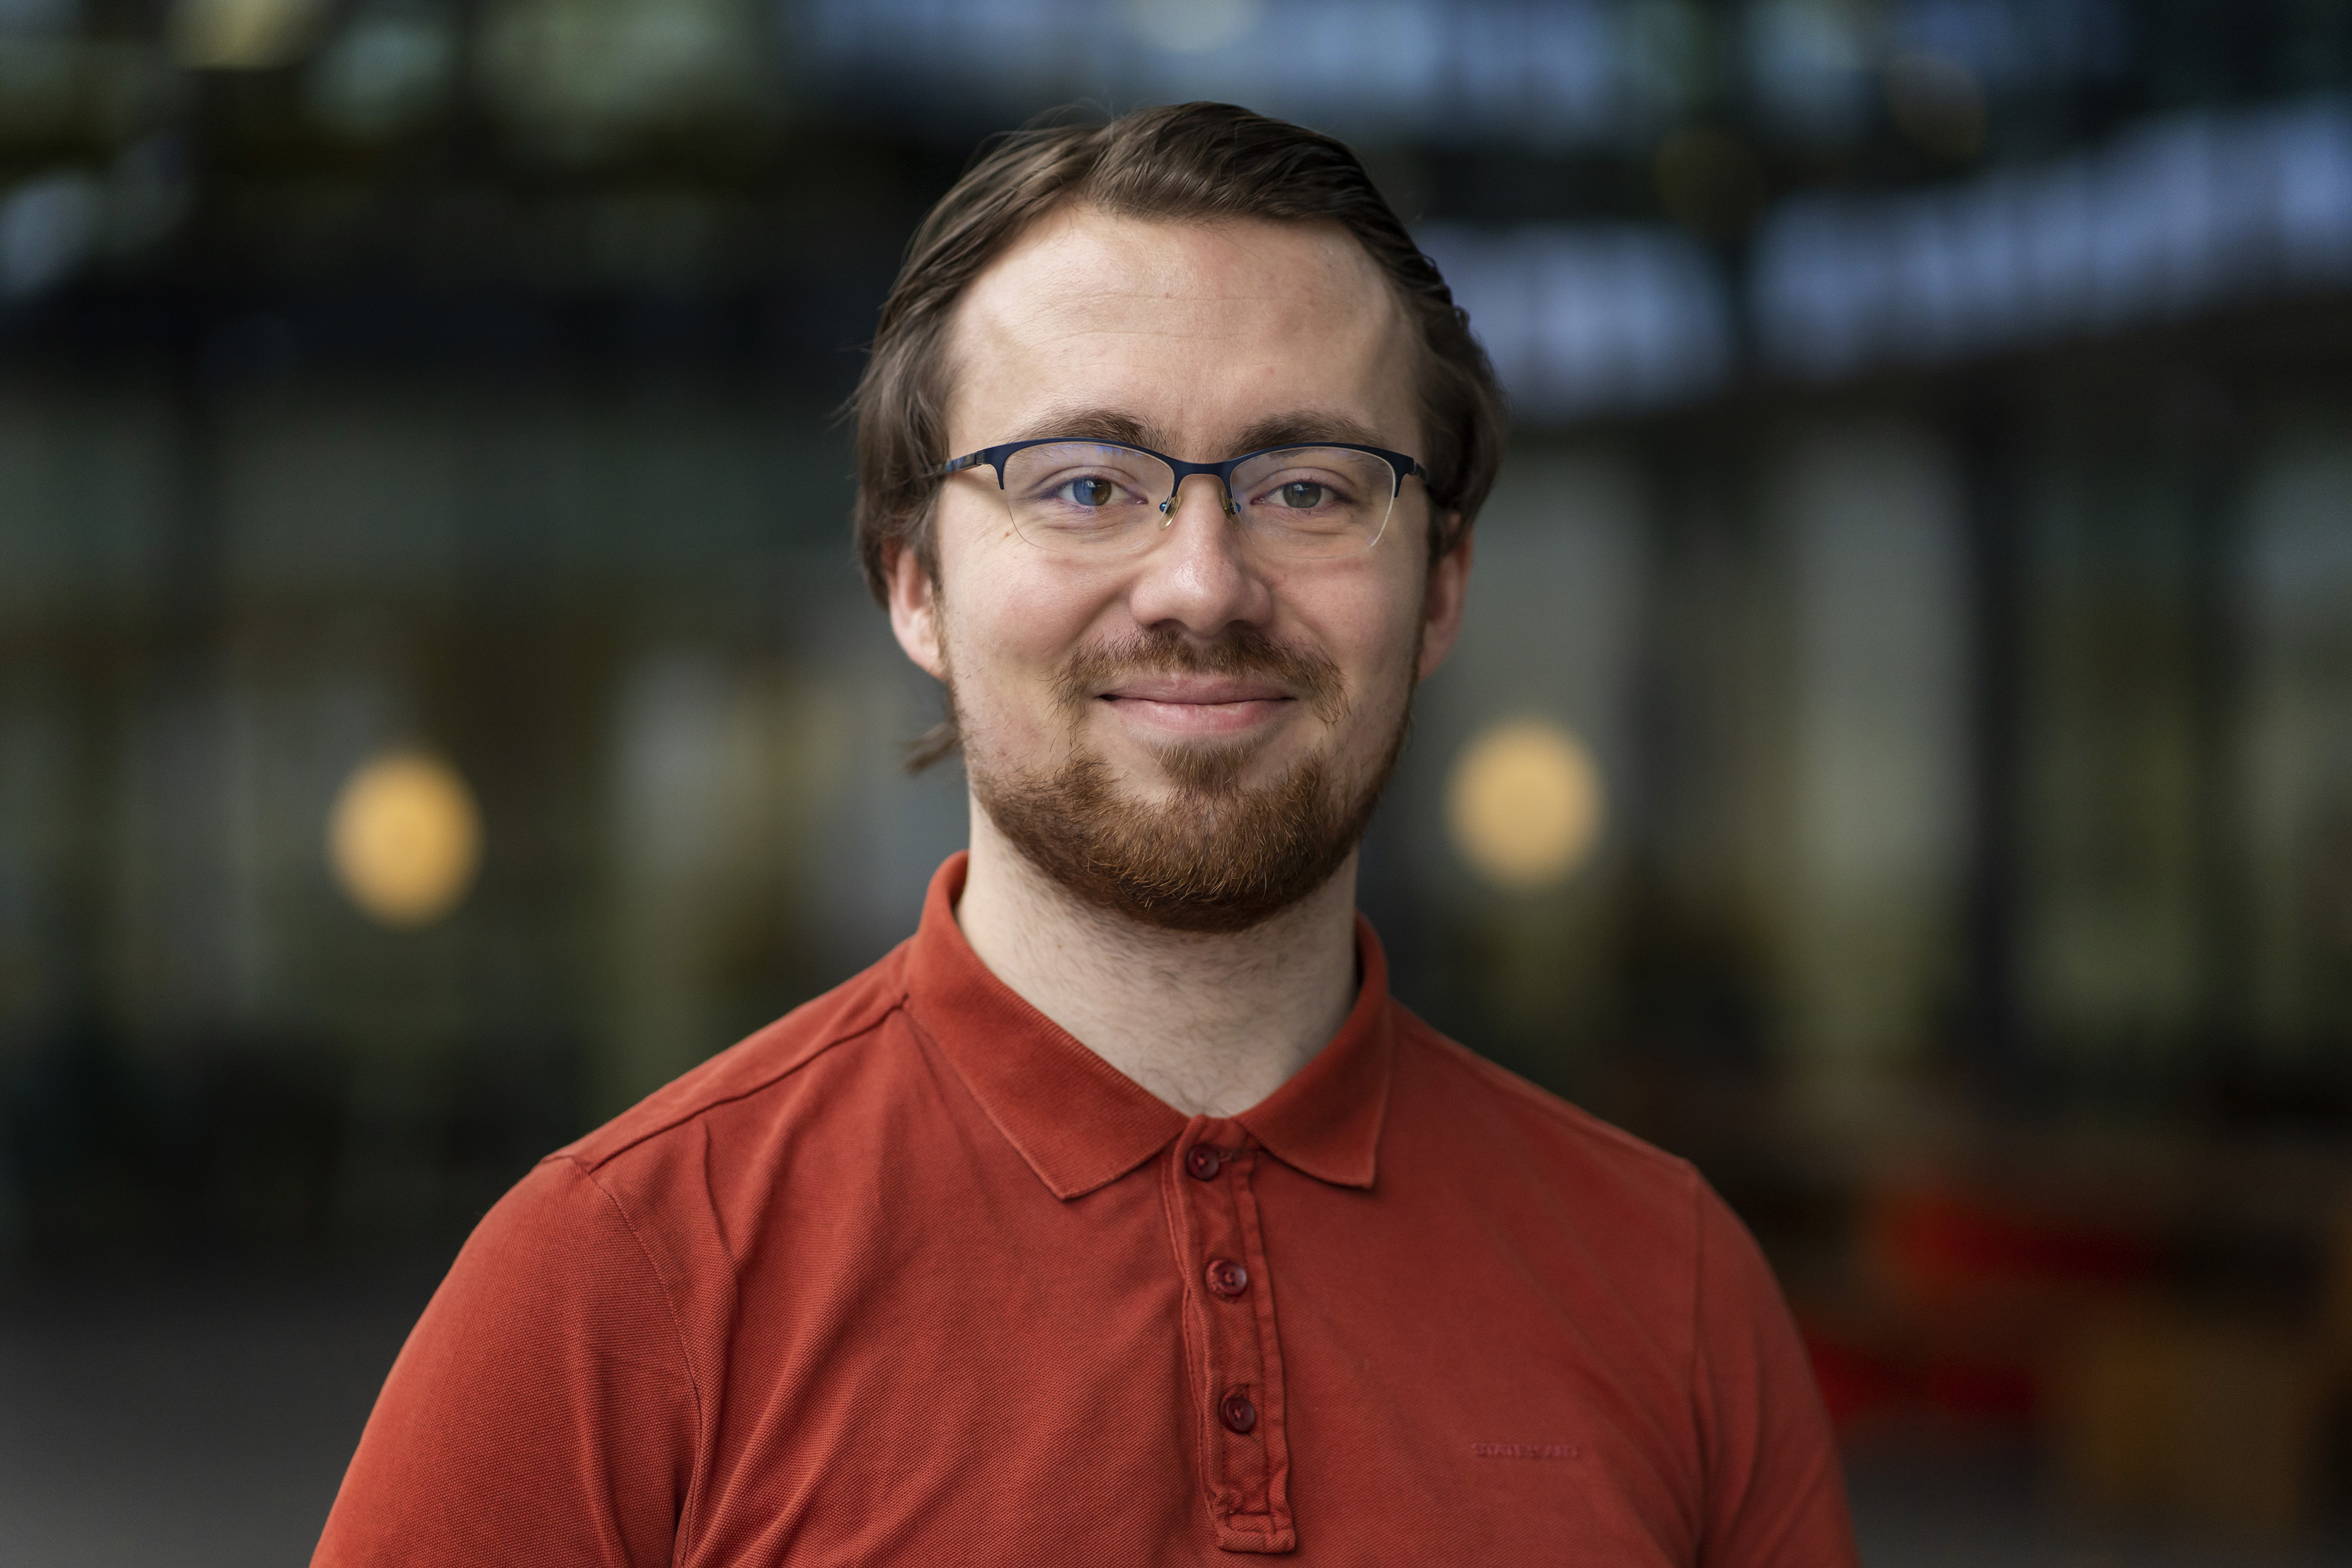
\includegraphics[height=140px, right, trim={4cm 0 6cm 0},clip]{Tom Franken.jpg}
		\end{subfigure}
	\end{figure}
	\noindent\rule{\textwidth}{0.4pt}
	\section*{Personal Profile}
	\noindent Currently finishing my Computer Science Master, my main interests lie with the fields Algorithms and Formal System Analysis. Currently, I am orientating for a PhD position, as going deeper into the research and development of new techniques interests me to no end.
	\ \\\ \\\ \\
	\noindent\rule{\textwidth}{0.4pt}
	\section*{Area's of Interest}
	\begin{itemize}[noitemsep, nolistsep]
		\item Algorithms
		\begin{itemize}
		\item Uncertainty
		\item Subtrajectory Clustering/Covering
		\item The Fréchet Distance
		\end{itemize}
		\item Formal Systems Analysis
		\begin{itemize}
			\item Logic \& Set Theory
			\item Algorithms for Model Checking
		\end{itemize}
	\end{itemize}
	\ \\\ \\
	\noindent\rule{\textwidth}{0.4pt}
	\section*{Education}
	\begin{itemize}
		\item \underline{Technical University Eindhoven, Master Computer Science} \hfill \textit{\color{Blue}{09/2018-08/2021}}
		\begin{itemize}[noitemsep, nolistsep]
		\item Software Science Stream
		\item \emph{Final Project:}
		\begin{itemize}
		\item \textbf{Subtrajectory Covering with Free Space Grids} \emph{(title subject to change)}
		\begin{itemize}
		\item \emph{Subject}: How to create a data structure containing a set system oracle for use in solving Subtrajectory Covering with Greedy Set Cover, with focus on Free Space Grids as used when working with the Fréchet Distance.
		\item \emph{Supervisors}: Associate Professor Kevin Buchin (Technical University Eindhoven), Professor Anne Driemel (University Bonn).
		\end{itemize}
		\end{itemize}
		\item Electives: focus on Algorithms \& Formal Systems Analysis Courses
		\item \emph{Internship} \emph{(extra)}:
		\begin{itemize}
		\item \emph{Subject}: Formally translating Hierarchical Equation Systems into Parameterized Boolean Equation Systems and the use of CHC solving on both HES and its equivalent PBES.
		\item \emph{Supervisor}: Tim Willemse (Technical University Eindhoven)
		\end{itemize}
		\end{itemize}
		\newpage
		\item \underline{Technical University Eindhoven, Bachelor Computer Science} \hfill \textit{\color{Blue}{09/2015-07/2018}}
		\begin{itemize}[noitemsep, nolistsep]
			\item Combined Majors Software Science \& Web Science
			\item \textit{Bachelor End Project:}
			\begin{itemize}[noitemsep, nolistsep]
				\item The development of the \textbf{Soccer Robot Remote} for Tech United, the autonomous Soccer Robot Team of the TU/e. Includes the development of a frontend with React and styled-components (tested with Jest), a backend with Go and JSON and the production of several official documents and documentation for the Soccer Robot Remote.
			\end{itemize}
			\item \textit{Electives:}
			\begin{itemize}[noitemsep, nolistsep]
				\item Courses on Graphics and Artificial Intelligence
				\item Courses on Entrepreneurship
			\end{itemize}
		\end{itemize}
		\item \underline{Stedelijk Gymnasium Den Bosch (SGDB)} \hfill \textit{\color{Blue}{09/2009-07/2015}}
		\begin{itemize}[noitemsep, nolistsep]
			\item \textit{Profile:} Nature \& Technology and Nature \& Health
			\item \textit{Notable Electives:}
			\begin{itemize}[noitemsep, nolistsep]
				\item German
		%		\item Art/Music
		%		\item Biology
		%		\item Computer Science
			\end{itemize}
		\end{itemize}
		%\item Primary School \hfill \textit{\color{Blue}{$<$07/2009}}
	\end{itemize}
	\ \\\ \\
	\noindent\rule{\textwidth}{0.4pt}	
	\section*{Work Experience}
	\begin{itemize}
		\item At the Technical University Eindhoven:
		\begin{itemize}
			\item Student Assistant Logic \& Set Theory\hfill \textit{\color{Blue}{09/2017-10/2017 \& 09/2020-11/2020}}\\
				\textit{\color{darkgray}{During this course, I graded weekly tests and tutored a group of students.}}
			\item Student Assistant Algorithms\hfill \textit{\color{Blue}{11/2018-01/2019 \& 09/2019-11/2019}}\\
				\textit{\color{darkgray}{During this course, I helped grading the weekly homeworks and assisted at the weekly tutorial sessions.}}
			\item Student Assistant Computer Systems\hfill \textit{\color{Blue}{02/2018-04/2018}}\\
				\textit{\color{darkgray}{During this course, I helped during the practical sessions by answering questions and judging when a group completed an exercise. Additionally, I monitored the chat during the streaming of lectures and helped with making the streaming experience smoother.}}\\\ \\
	\end{itemize}
	\end{itemize}
	\noindent\rule{\textwidth}{0.4pt}	
	\newpage
	\noindent\rule{\textwidth}{0.4pt}	
	\section*{Other Experiences}
	\begin{itemize} [noitemsep]
		
		%	\textit{\color{Blue}{I assist in the Sunday service. Since recently, I also read certain parts during the service.}}
		\item Active Member of Da Vinci, Archery Association Eindhoven  \hfill \textit{\color{Blue}{09/2015-now}}
		\item Secretary of Da Vinci, Archery Association Eindhoven \hfill \textit{\color{Blue}{11/2016-10/2017, 10/2020-now}}
		\item Member of Student Team T.E.S.T. (TU/e Sensing Team)\hfill \textit{\color{Blue}{11/2017-09/2018}}\\
		\textit{\color{darkgray}{T.E.S.T. is a team competing in the SensUs competition, organized by TU/e students. The goal is to create a biosensor to detect an antibody (which was chosen to be Vancomycin in my year). I have been involved in the market research and the Software and Hardware of the envisioned biosensor.}}
		%\item Saturday machinery cleaning job at a butcher \hfill \textit{\color{Blue}{09/2014-12/2017}}\\
		%	\textit{\color{Blue}{I cleaned two machines, machine parts, plates, cutlery and several other things with specialized tools.}}
		%\item Kitchen Employee at the Jeroen Bosch Hospital, Den Bosch \hfill \textit{\color{Blue}{08/2013, 08/2014}}\\
		%	\textit{\color{darkgray}{I helped with the composition of meals, which meant around 2 or 3 times about 2 or 3 hours of food assembly line work.}}
		%\item Internal Postman at the Jeroen Bosch Hospital, Den Bosch \hfill \textit{\color{Blue}{08/2013}}\\
		%	\textit{\color{Blue}{The job concerned the sorting and delivery of post throughout the hospital.}}
		%\item Member (Keyboard/Piano) of the SGDB School Orchestra, Mercator \& Musica \hfill \textit{\color{Blue}{09/2009-07/2015}}\\
		%	\textit{\color{darkgray}{We made music as an orchestra during the year, the highlight being the Orkestival in the Royal Concertgebouw in Amsterdam.}}
		%\item Participant of several iterations of the Musical (Orchestra) at the SGDB, Den Bosch \hfill \textit{\color{Blue}{09/2010-04/2015}}\\
		%	\textit{\color{darkgray}{I was part of the orchestra and played keys. We were responsible for all musical accompaniment during the performance.}}
		%\item Member of the SGDB Model European Parliament Team\hfill \textit{\color{Blue}{04/2013}}\\
		%	\textit{\color{darkgray}{A week of debating and imitating European Politics, each team with their own goals, suits and real facts. Included several excursions about politics and europe.}}
		%\item Lector at the St. Lambertus Church, Den Bosch \hfill \textit{\color{Blue}{2004-now}}\\
	\end{itemize}
	\ \\\ \\
	\noindent\rule{\textwidth}{0.4pt}
	\section*{Skills, Competences, Hobbies and Sports}
	\begin{figure}[h]
		\begin{subfigure}[t]{0.5\textwidth}
			\vskip 0pt
			\subsection*{Languages}
			\begin{itemize}[noitemsep]
				\item Dutch, \textit{native language}
				\item English, \textit{advanced}
				\item German, \textit{high school level}
			\end{itemize}
			\subsection*{Attributes}
			\begin{itemize}[noitemsep]
				\item Flexible and focused
				\item Continuously looking for ways to develop
				\item Interested in both the theory and the application
				\item Dedicated to the task at hand
			\end{itemize}	
		\end{subfigure}
		\begin{subfigure}[t]{0.5\textwidth}
			\vskip 0pt
			\subsection*{Programming Languages}
			\begin{itemize}[noitemsep]
				\item Java, \textit{advanced}
				\item Python, \textit{advanced}
				\item \LaTeX, \textit{advanced}
				\item HTML/CSS/JavaScript \& React, \textit{intermediate}
				\item C, \textit{beginner}
				\item C++, \textit{beginner}
				\item Go, \textit{beginner}
				\item JSON, \textit{beginner}
				\item SQL, \textit{beginner}
				\item Rascal, \textit{beginner}
			\end{itemize}
		\end{subfigure}
		\begin{subfigure}[t]{0.5\textwidth}
			\vskip 10pt
			\subsection*{Sports}
			\begin{itemize}[noitemsep]
				\item Archery
				\item Walking
				\item Bicycling
				\item Swimming
				\item Dancing
			\end{itemize}
		\end{subfigure}
		\begin{subfigure}[t]{0.5\textwidth}
			\vskip 10pt
			\subsection*{Hobbies}
			\begin{itemize}[noitemsep]
				\item Reading
				\item Music
				\item Digital Drawing
				\item Board- and Roleplaying Games
			\end{itemize}
		\end{subfigure}
	\end{figure}
	\ \\\ \\
	\noindent\rule{\textwidth}{0.4pt}
\end{document}